\ffigbox[\FBwidth]{%
\label{Fig:dm1ex1}
}{
    \fbox{
        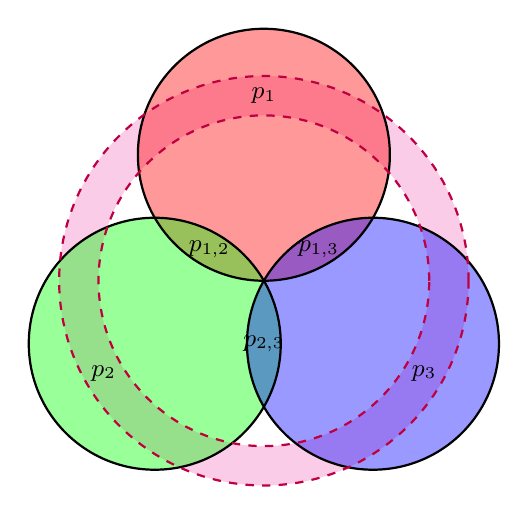
\begin{tikzpicture}[scale=1, every node/.style={circle, draw, fill=blue!20, inner sep=1pt, font=\scriptsize, minimum size=4mm}]
            % centers of the three circles
            \coordinate (A) at (90:1.6cm);
            \coordinate (B) at (210:1.6cm);
            \coordinate (C) at (330:1.6cm);
            \def\r{1.6cm} % radius (adjust as desired)
            
            % Add the circular band/strip
            \def\bandInnerRadius{2.1cm}
            \def\bandOuterRadius{2.6cm}

            % Draw the band with some transparency
            \fill[magenta, fill opacity=0.2] (0,0) circle (\bandOuterRadius);
            \fill[white] (0,0) circle (\bandInnerRadius);

            % draw filled circles with transparency
            \fill[red,   fill opacity=0.4]  (A) circle (\r);
            \fill[green, fill opacity=0.4]  (B) circle (\r);
            \fill[blue,  fill opacity=0.4]  (C) circle (\r);

            % remove (mask out) the triple-intersection area
            \begin{scope}
                \clip (A) circle (\r);
                \clip (B) circle (\r);
                \clip (C) circle (\r);
                % filling a large rectangle inside the triple-clip erases that area
                \fill[white] (-3,-3) rectangle (3,3);
            \end{scope}

            % circle outlines
            \draw[line width=0.8pt] (A) circle (\r);
            \draw[line width=0.8pt] (B) circle (\r);
            \draw[line width=0.8pt] (C) circle (\r);
            
            % Optional: Add outline for the band
            \draw[line width=0.8pt, purple, dashed] (0,0) circle (\bandInnerRadius);
            \draw[line width=0.8pt, purple, dashed] (0,0) circle (\bandOuterRadius);

            % Updated labels - moved to intersections between strip and circles
            \node[circle, draw=none, fill=none, font=\small] at (90:2.35cm) {\(p_1\)}; % Top circle
            \node[circle, draw=none, fill=none, font=\small] at (210:2.35cm) {\(p_2\)}; % Bottom left circle
            \node[circle, draw=none, fill=none, font=\small] at (330:2.35cm) {\(p_3\)}; % Bottom right circle

            % Labels for pairwise intersections (unchanged)
            \node[circle, draw=none, fill=none, font=\small] at (30:0.8cm) {\(p_{1,3}\)}; % A∩C
            \node[circle, draw=none, fill=none, font=\small] at (150:0.8cm) {\(p_{1,2}\)}; % A∩B
            \node[circle, draw=none, fill=none, font=\small] at (270:0.8cm) {\(p_{2,3}\)}; % B∩C
        \end{tikzpicture}
    }
}